\chapter{适应其世界}\label{ch:g4:adapted-to-their-world}

把北极熊放到撒哈拉沙漠，把骆驼放到浮冰上，两者
都撑不过一个季节。可各自在家乡都是能手：北极熊
在冰冷的海里游得从容自如，骆驼穿越的沙漠，
几天就能把一匹马累垮。\omterm{def:g1:living-or-not:living}{生物}与其所处的世界彼此契合，
精确得值得细究——一处特征
接着一处特征地看。

\section{适应的含义}

\begin{definition}[适应]\label{def:g4:adapted-to-their-world:adaptation}
\emph{适应}\index{适应}是一种\omterm{def:g1:living-or-not:living}{生物}体身体或行为上的特征，
它使\omterm{def:g1:living-or-not:living}{生物}能够适应其\omterm{def:g2:caring-for-nature:environment}{环境}的条件——
即寒冷或干旱、食物、
天敌。\Cref{prop:g2:where-animals-live:fit}说明了
\omterm{def:g1:animals-around-us:animal}{动物}如何与其\omterm{def:g2:where-animals-live:habitat}{栖息地}相契合；适应就是
逐项细看这种契合。
\end{definition}

\begin{example}[骆驼，逐项来看]\label{ex:g4:adapted-to-their-world:camel}
沙漠的难题：炎热、缺水、沙子松软。骆驼的应对
：驼峰里储存脂肪，作为长途跋涉时的食物储备；
能在几分钟内喝下一百升水，然后
数日不饮；宽阔的双趾脚掌，不会陷入沙中；
鼻孔能够闭合，以挡住飞扬的风沙，还有长而密的双层
睫毛与之配合。每一个沙漠难题，都由一种特征来应对。
\end{example}

\begin{omfigure}
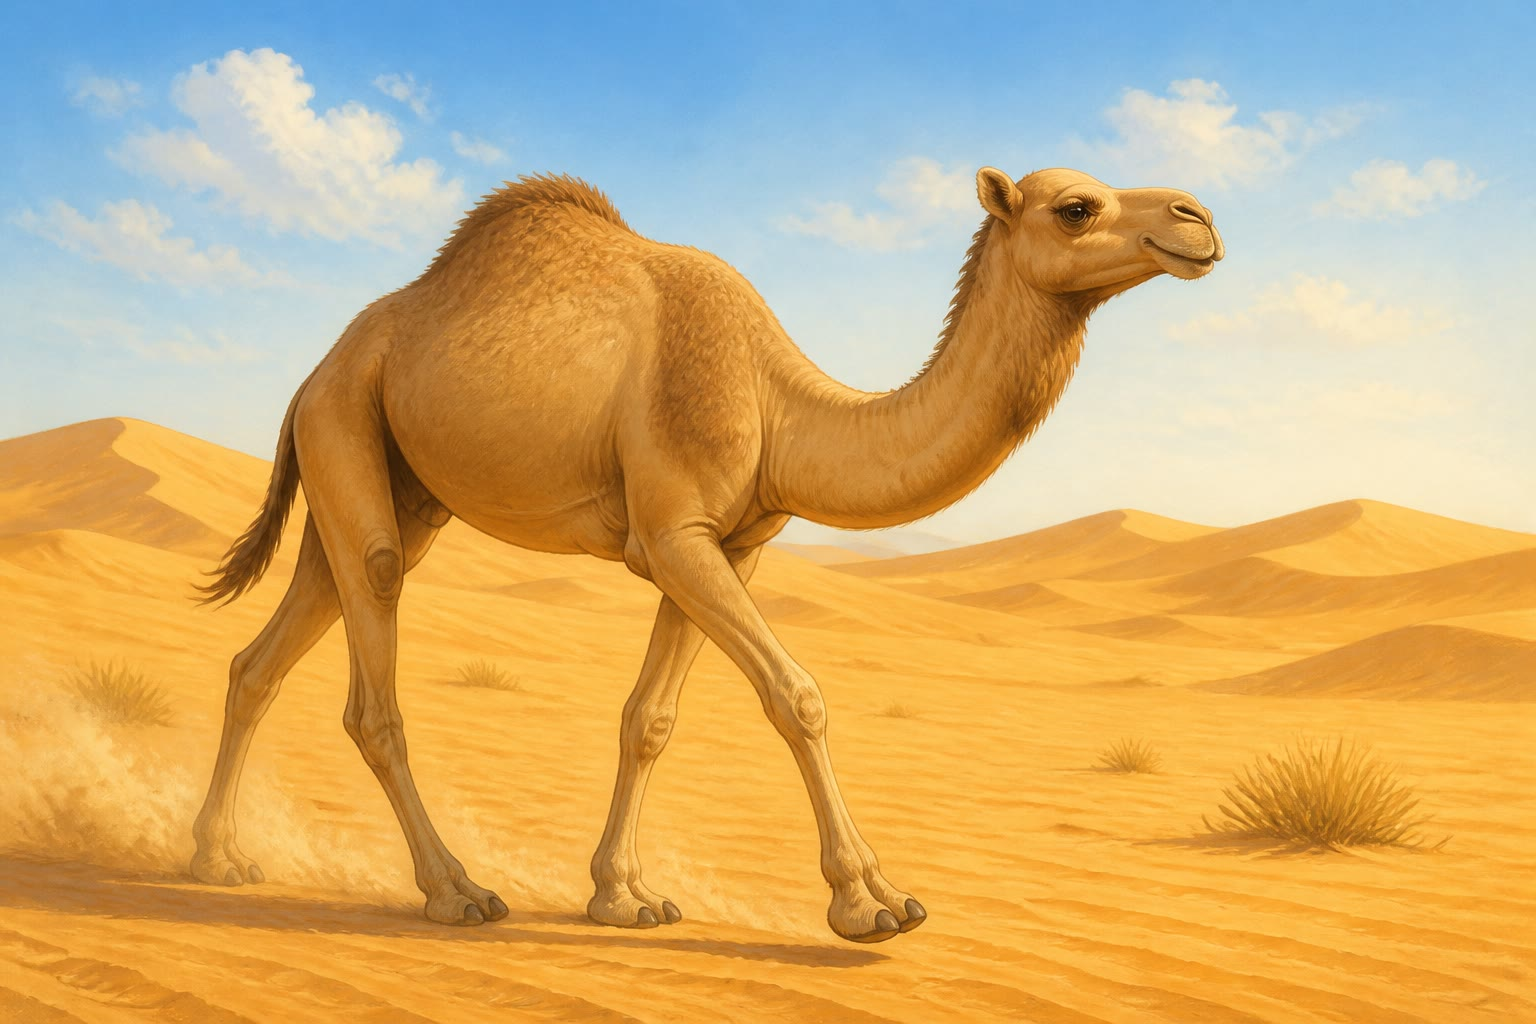
\includegraphics[width=0.6\linewidth]{images/book1/ai/g4-adapted-camel.jpg}

{\small 沙漠里的专家在工作：宽阔的脚掌踩在松软的沙上，
驼峰是储备，睫毛是为挡风沙而生。}
\end{omfigure}

\begin{example}[北极熊，逐项来看]\label{ex:g4:adapted-to-their-world:bear}
浮冰的难题：寒冷、冰冷的海水，以及
在白色冰面上难以靠近的猎物。北极熊的应对：厚厚的毛皮之下
是一层厚厚的脂肪，形成双重保温；宽阔而略带蹼的
爪子，既是雪地鞋，又是划水的桨；白色的\omterm{def:g1:animals-around-us:covering}{皮毛}，
在它捕猎的雪地上几乎隐形。同样的精确，
只是调校到了相反的世界。
\end{example}

\begin{proposition}[适应应对难题]\label{prop:g4:adapted-to-their-world:answers}
\omterm{def:g2:caring-for-nature:environment}{环境}中每出现一种严峻的难题，当地的
\omterm{def:g1:living-or-not:living}{生物}便会带有能够应对它的特征：
\begin{itemize}
  \item 寒冷：厚厚的毛皮、脂肪层、
        散热少的小耳朵；
  \item 干旱：储水、蜡质的\omterm{def:g1:the-five-senses:sense}{皮肤}、深扎的根；
  \item 水中生活：流线型身体、鳍和蹼状的
        脚、防水的\omterm{def:g1:animals-around-us:covering}{皮毛}；
  \item 四周有天敌：保护色、护甲、刺、
        速度，以及两眼分开、便于四面观察；
  \item 靠捕猎谋生：敏锐的感觉、朝前的眼睛、
        利爪和速度
        （\cref{prop:g2:what-animals-eat:match}）。
\end{itemize}
\end{proposition}
\admitted

\section{植物也有适应}

\begin{example}[仙人掌]\label{ex:g4:adapted-to-their-world:cactus}
沙漠对\omterm{def:g1:plants-around-us:plant}{植物}的考验最为严酷——它们无法走到
水源边。仙人掌的应对：粗壮、呈桶状的茎，
既储存水分，又承担叶片的捕光工作；\omterm{def:g1:plants-around-us:parts}{叶子}
缩成刺，几乎不散失水分，同时还能保护
那只“水桶”，防止口渴的\omterm{def:g1:animals-around-us:animal}{动物}啃食；\omterm{def:g1:plants-around-us:parts}{根系}
向四周浅浅地铺开，一场珍贵的阵雨来临时便能尽数吸收。
\end{example}

\begin{example}[高山垫状植物]\label{ex:g4:adapted-to-their-world:alpine}
高山\omterm{def:g1:plants-around-us:plant}{植物}要面对刺骨的寒风。许多\omterm{def:g1:plants-around-us:plant}{植物}长成紧贴
地面的致密垫子：垫子内部风被挡住，
空气保持温和——这种形态本身就是一座庇护所。
同种\omterm{def:g1:plants-around-us:plant}{植物}的低地近亲则长得高而松散；
高山上的垫状\omterm{def:g1:plants-around-us:plant}{植物}则紧贴岩石。
\end{example}

\begin{method}[从生物的身体读出其所处的世界]\label{met:g4:adapted-to-their-world:read}
给定一种不熟悉的\omterm{def:g1:animals-around-us:animal}{动物}或\omterm{def:g1:plants-around-us:plant}{植物}：
\begin{enumerate}
  \item 列出其显著的特征——\omterm{def:g1:animals-around-us:covering}{皮毛}、脚、眼睛、身体
        形状、\omterm{def:g1:plants-around-us:parts}{叶子}、根；
  \item 对每一项提问：\emph{这种特征能解决什么问题？}
  \item 把答案拼合成对其家园的图景——
        寒冷还是炎热、潮湿还是干燥、捕食者还是被捕食者；
  \item 将推测与该\omterm{def:g1:living-or-not:living}{生物}真正生活的
        地方对照检验。
\end{enumerate}
这是\cref{met:g2:where-animals-live:matching}的进阶版：
即从为\omterm{def:g2:where-animals-live:habitat}{栖息地}配对，发展到重构一个世界。
\end{method}

\begin{example}[用此方法辨认一张神秘的兽皮]\label{ex:g4:adapted-to-their-world:mystery}
博物馆的抽屉里有一张没有标签的兽皮：致密柔软的毛，
细小的眼睛，巨大的铲状前爪。有毛，说明是\omterm{prop:g3:sorting-living-things:groups}{哺乳动物}；
铲子般的爪说明它会挖掘；用不上的眼睛说明它生活在
黑暗之中。结论：一种地下挖掘者——它确实是
鼹鼠（\cref{ex:g2:where-animals-live:mole}），仅凭
三项特征就被正确读出。
\end{example}

\begin{remark}[契合是怎样形成的？]\label{rem:g4:adapted-to-their-world:how}
骆驼从不会\emph{决定}长出宽阔的脚掌，北极熊也从不
会选择自己白色的\omterm{def:g1:animals-around-us:covering}{皮毛}。那么，\omterm{def:g1:living-or-not:living}{生物}是如何
如此恰当地契合其世界的呢？这是生物学最深刻的
问题之一，它的完整答案——契合如何逐步积累，
一代又一代地形成——是本书留待
以后讲的内容。眼下，请学会\emph{看出}这种契合：
正是这种观察，使这个问题得以被提出。
\end{remark}

\section{练习}

\begin{exercise}[$\star$]\label{exo:g4:adapted-to-their-world:1}
什么是\omterm{def:g4:adapted-to-their-world:adaptation}{适应}？请举出一个\omterm{def:g1:animals-around-us:animal}{动物}例子和一个
\omterm{def:g1:plants-around-us:plant}{植物}例子。
\end{exercise}

\begin{exercise}[$\star$]\label{exo:g4:adapted-to-their-world:2}
说出沙漠中的三个问题，以及骆驼对每个问题的应对方式。
\end{exercise}

\begin{exercise}[$\star$]\label{exo:g4:adapted-to-their-world:3}
说出浮冰上的三个问题，以及北极熊
对每个问题的应对方式。
\end{exercise}

\begin{exercise}[$\star$]\label{exo:g4:adapted-to-their-world:4}
仙人掌的刺有什么作用？它的桶状茎
储存了什么？茎又接替了哪项工作？
\end{exercise}

\begin{exercise}[$\star$]\label{exo:g4:adapted-to-their-world:5}
为什么许多高山\omterm{def:g1:plants-around-us:plant}{植物}长成紧密的垫状？
\end{exercise}

\begin{exercise}[$\star$]\label{exo:g4:adapted-to-their-world:6}
列出被猎\omterm{def:g1:animals-around-us:animal}{动物}和猎食者各两种\omterm{def:g4:adapted-to-their-world:adaptation}{适应}，
出处见\cref{prop:g4:adapted-to-their-world:answers}。
\end{exercise}

\begin{exercise}[$\star$]\label{exo:g4:adapted-to-their-world:7}
复述\cref{ex:g4:adapted-to-their-world:mystery}：哪三个
特征暴露了鼹鼠，每个特征
分别说明了什么？
\end{exercise}

\begin{exercise}[$\star$]\label{exo:g4:adapted-to-their-world:8}
动手试一试：任选一种你能观察的\omterm{def:g1:animals-around-us:animal}{动物}，
如鸭子、猫或蜘蛛，并对它运行
\cref{met:g4:adapted-to-their-world:read}，找出
三个特征，说明它解决的三个问题。
\end{exercise}

\begin{exercise}[$\star\star$]\label{exo:g4:adapted-to-their-world:9}
沙漠狐的耳朵极大，北极狐的耳朵极小。
请利用关于寒冷的那一条，
\cref{prop:g4:adapted-to-their-world:answers}中的内容解释这两种情况——
大耳朵要如何处理热量？
\end{exercise}

\begin{exercise}[$\star\star$]\label{exo:g4:adapted-to-their-world:10}
一种神秘\omterm{def:g1:animals-around-us:animal}{动物}：身体呈流线型，后足有蹼，
\omterm{def:g1:animals-around-us:covering}{皮毛}浓密且防水，有胡须，并且能长时间憋气。
请运用
\cref{met:g4:adapted-to-their-world:read}重建它的生存\omterm{def:g2:caring-for-nature:environment}{环境}。（它会筑坝。）
\end{exercise}

\begin{exercise}[$\star\star\star$]\label{exo:g4:adapted-to-their-world:11}
鲸（\cref{ex:g3:sorting-living-things:surprises}）是一种外形像鱼的\omterm{prop:g3:sorting-living-things:groups}{哺乳动物}：
身体流线型，有鳍，表面光滑。鳟鱼也是外形相同的鱼。这两种
\emph{互不相关}的游泳\omterm{def:g1:animals-around-us:animal}{动物}之间的相似之处说明了\omterm{def:g4:adapted-to-their-world:adaptation}{适应}的什么问题？
决定这种外形的是谁？
是亲缘关系，还是水\omterm{def:g2:caring-for-nature:environment}{环境}？
\end{exercise}
